\documentclass[a4paper,12pt]{article}

\renewcommand{\labelenumii}{\theenumii}
\renewcommand{\theenumii}{\theenumi.\arabic{enumii}.}

\usepackage[T2A]{fontenc}
\usepackage[utf8]{inputenc}
\usepackage[english,russian]{babel}
\usepackage{hyperref}
\usepackage{graphicx}
\graphicspath{{lab2_images/}}
\usepackage[a4paper, total={8in, 10in}]{geometry}

\begin{document}
	\begin{enumerate}
		\item \begin{enumerate}
			\item Как устроен стековый фрейм на x86\_64 для System V ABI?\\
			\textbf{Ответ:}\\
			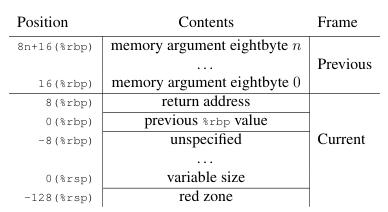
\includegraphics{stack_frame.jpg}\\
			Стэк растёт от старших адресов к младшим.
			
			\item Как передаются аргументы?\\
			\textbf{Ответ:}\\
			
			
			\item Как получить возвращаемое значение из функции?\\
			\textbf{Ответ:}\\
			
			
			\item Восстановление стек трейса, как можно реализовать в программе?\\
			\textbf{Ответ:}\\
			
			
			\item Как узнать, когда перестать раскручивать фрейм?\\
			\textbf{Ответ:}\\
			
			
			\item Что можно сделать, если код не выделяет стековый фрейм явным образом\\ (-fomit-frame-pointer)?\\
			\textbf{Ответ:}\\
			
			
		\end{enumerate}
	\item \begin{enumerate}
		\item Где аллоцируется стек ядра, стек прошивки?\\
		\textbf{Ответ:}\\
		
		
		\item Когда JOS использует тот или иной стек, когда перестаёт использовать стек прошивки?\\
		\textbf{Ответ:}\\
		
		
		\item Всегда ли стек доступен?\\
		\textbf{Ответ:}\\
		
		
		\item Почему нельзя переиспользовате стек прошивки в ядре?\\
		\textbf{Ответ:}\\
		
		
		\end{enumerate}
	\item \begin{enumerate}
		\item Как запускается JOS на 32-битной прошивке UEFI?\\
		\textbf{Ответ:}\\
		
		
		\item В чём отличия от 64-битного запуска?\\
		\textbf{Ответ:}\\
		
		
		\item Зачем нужен head64 (bootstrap.S) при запуске JOS?\\
		\textbf{Ответ:}\\
		
		
		\item Можно ли было избежать его реализации (объединив его код с entry.S)?\\
		\textbf{Ответ:}\\
		
		
		\end{enumerate}
	\end{enumerate}
\end{document}